\documentclass[paper=a4, fontsize=11pt]{scrartcl} % A4 paper and 11pt font size

\usepackage[english]{babel} % English language/hyphenation
\usepackage{fancyhdr} % Custom headers and footers
\usepackage{graphicx}
\usepackage{xcolor}
\usepackage{titlesec}

\graphicspath{ {images/} }
\pagestyle{fancyplain}

\fancyhead{} 
\fancyfoot[L]{} % Empty left footer
\fancyfoot[C]{} % Empty center footer
\fancyfoot[C]{\thepage} % Page numbering for center footer
\renewcommand{\headrulewidth}{0pt} % Remove header underlines
\renewcommand{\footrulewidth}{0pt} % Remove footer underlines
\setlength{\headheight}{13.6pt} % Customize the height of the header
\titleformat{\section}[block]{\Large\bfseries\filcenter}{}{65pt}{}
\titleformat{\subsection}[hang]{\bfseries}{}{40pt}{}

\title {
	\normalfont \normalsize 
	\textsc{University of Pretoria, Department of Computer Science} \\ [25pt]
	\huge Scope, Vision, Non-Functional \& Functional Requirements Specification\\
}

\author {
	Brandon Wardley u29005150 \\
	Mothusi Masibi \\
	Marc Antel \\
	Stuart Andrews \\
}
\date{\normalsize\today} % Today's date or a custom date

\begin{document}
	\maketitle % Print the title
	\newpage
	\section{Vision}
	PowerCloud is a system which allows its users to measure the power consumption of an appliance, store this information on a cloud platform, and view useful reports based on this information via a web interface. The system will allow the storage of important metadata pertaining to a source's power consumption and which devices the data is taken from. The system is initially intended to be used for internal use and testing by the client, Bühler.\\
	
	The system will consist out of a hardware component, and a software component. The hardware component will be tasked with measuring the current and voltage from an input device, which will be used to perform the power calculations which are required. The hardware device will send this information to a web server. This server will perform any required processing on this information, before posting it to a persistence provider.\\
	
	A user within the system will have access to a number of functions. Users will be able to add and set up new devices, adding to the system, which will send data based on readings from the attached appliance. Additionally, the user can view the data once it has be stored on the persistence provider, and can request reports based off of this data.
	\newpage
	\section{Scope}
	\subsection{Device Management}
		\begin{figure}[H]
			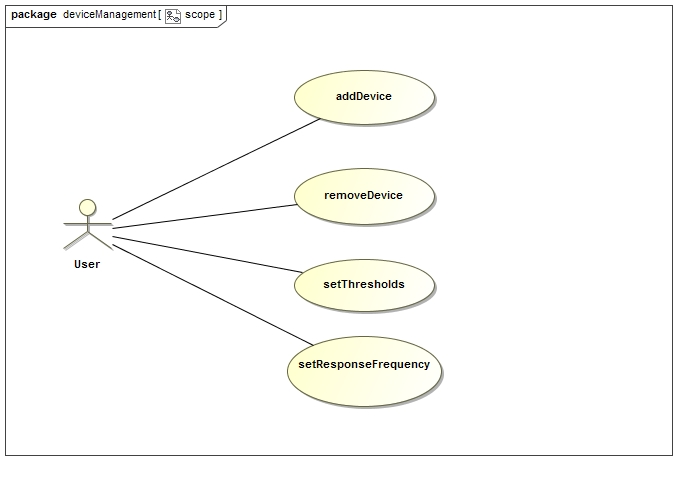
\includegraphics[width=\textwidth]{images/deviceManagementScope.jpg}  \\
			\caption{The scope of functionality required from the deviceManagement module}
		\end{figure}
		
		A user is able to add and register a new device onto the system, as well as remove old, unnecessary devices. The user can set the measurement thresholds for a specific device, and set how often the device should aim to transfer its data to the web server.
		
	\subsection{User Management}
		\begin{figure}[H]
			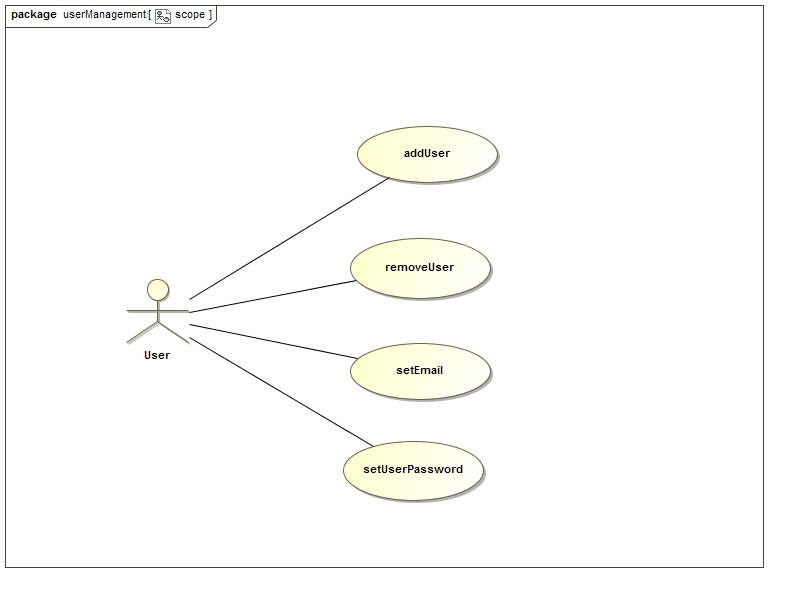
\includegraphics[width=\textwidth]{images/userManagementScope.jpg}  \\
			\caption{The scope of functionality required from the userManagement module.}
		\end{figure}
		
		A user is able to add other users to the system, as well as remove old or redundant users. A user can set their personal email address, as well as their password.
		
	\subsection{Data Management}
		\begin{figure}[H]
			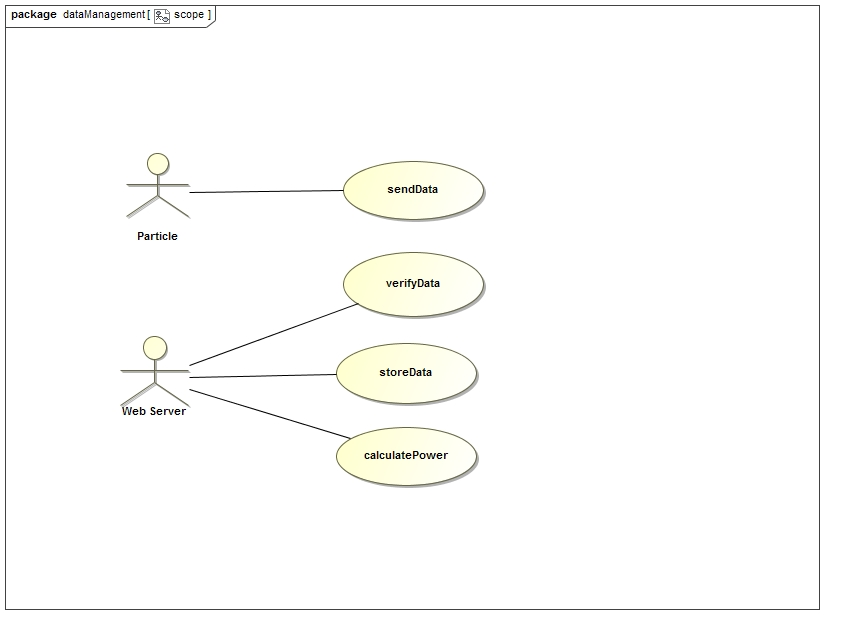
\includegraphics[width=\textwidth]{images/dataManagementScope.jpg}  \\
			\caption{The scope of functionality required from the dataManagement module.}
		\end{figure}
		
		The particle device will regularly send the data it has accumulated to the web server. The web server can verify the data which it receives, perform the necessary calculations on the received data to calculate desired values, and store the data and results to the persistence service.
		
	\subsection{Reporting Scope}
	\begin{figure}[H]
		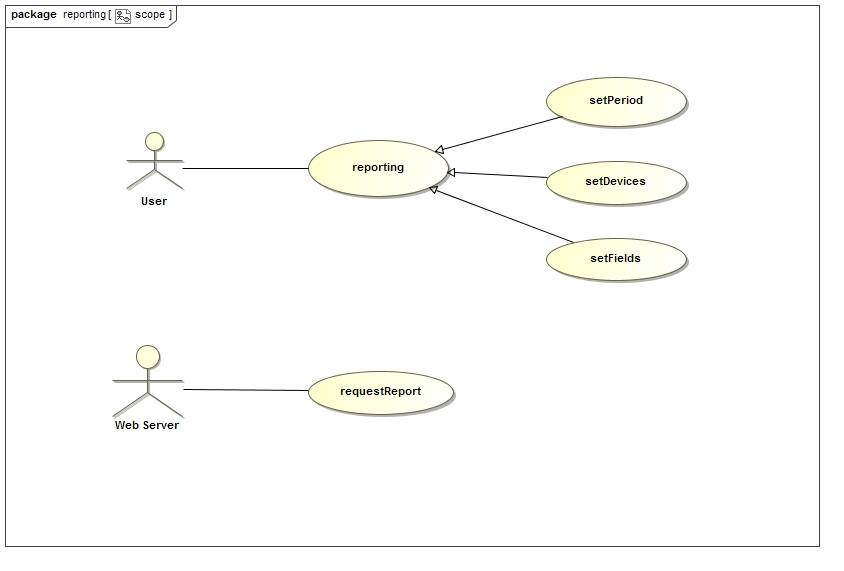
\includegraphics[width=\textwidth]{images/reportingScope.jpg}  \\
		\caption{The scope of functionality required from the reporting module.}
	\end{figure}
	
	The user can request a report made up of data from between a certain period of time, from a certain set of devices, containing a certain set of fields. The web server requests the report from the reporting service, which accesses the required data, compiles and returns the report to the web server.
	\newpage
	\section{Initial Architecture Design}
	\begin{figure}[H]
		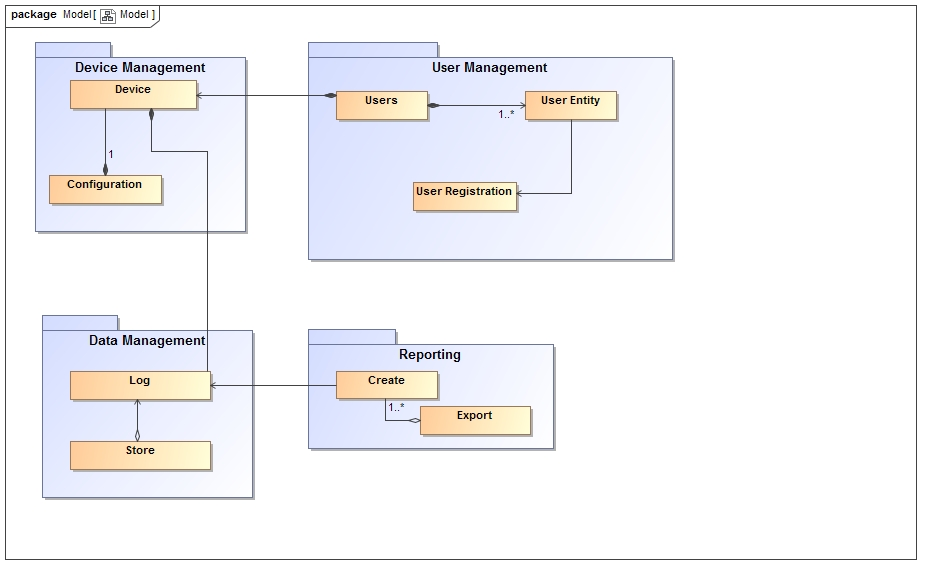
\includegraphics[width=\textwidth]{images/ArchitecturalModel.jpg}  \\
		\caption{The initial Domain Model}
	\end{figure}
	
	\begin{figure}[H]
		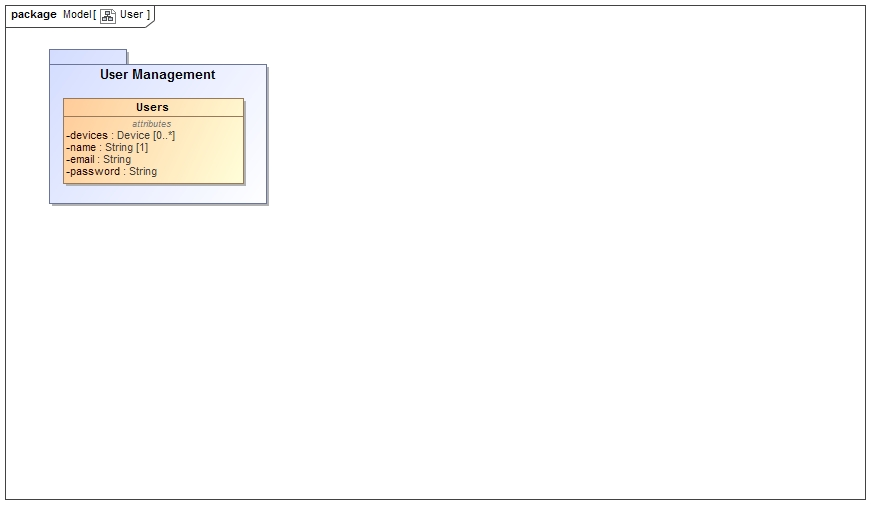
\includegraphics[width=\textwidth]{images/User.jpg}  \\
		\caption{The user package.}
	\end{figure}
	
	\begin{figure}[H]
		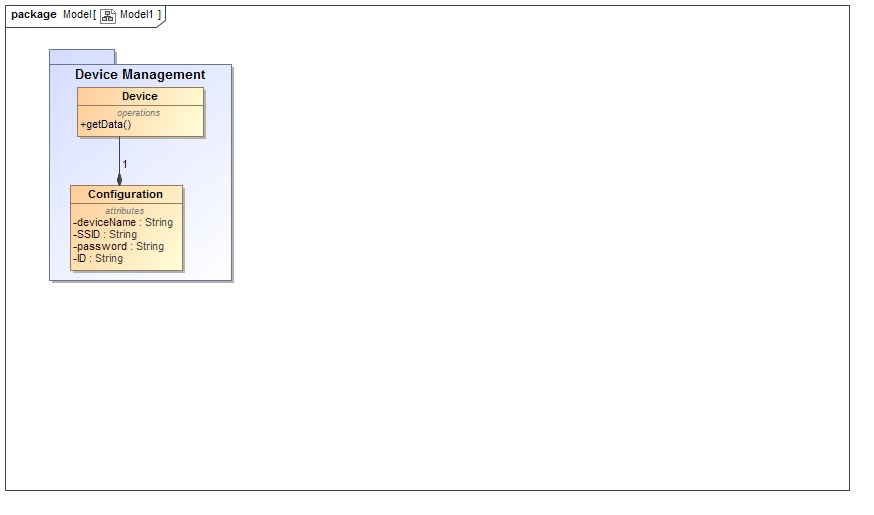
\includegraphics[width=\textwidth]{images/DeviceManagement.jpg}  \\
		\caption{The device management package.}
	\end{figure}
	
	\begin{figure}[H]
		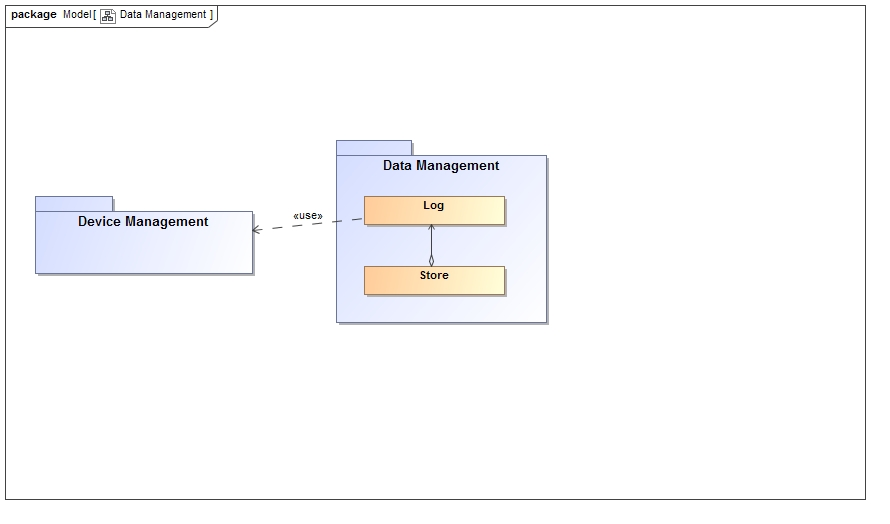
\includegraphics[width=\textwidth]{images/DataManagement.jpg}  \\
		\caption{The data management package.}
	\end{figure}
	
	\begin{figure}[H]
		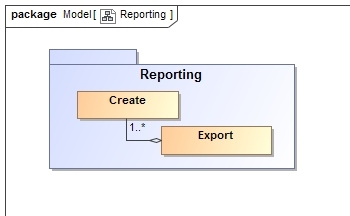
\includegraphics[width=\textwidth]{images/Reporting.jpg}  \\
		\caption{The reporting package.}
	\end{figure}
	\newpage
	\section{Functional Requirements}
	\newpage
	\section{Non-functional Requirements}
	\subsection{Quality requirements}
	Scalability: Server needs to handle up to 100 000 simultaneous connections.\\
	\\Reliability: The entire system should be portable to endure close to 100% up
	time.\\
	\\Quality: Server needs to ensure that data is valid and consistent.\\
	\\Recoverability: If the device goes offline, data should not be lost.\\
	Security: Security of devices should be handled to prevent unauthorized
	devices to log data.
	\newpage
	\section{Proposed Frameworks and Technologies}
	\subsection{Current transformer data transfers}
	Serial Peripheral Interface (SPI) will be used to send data to the photon. SPI is used as a synchronous data bus,
	and uses seperate lines for data and a clock which keeps both sides of the SPI in sync. The receiver (particle photon) detects an incoming 
	edge and will immediately data line.\\
	\\There are no alternatives to this technology.
	\subsection{Particle Photon}
	The Photon has built in functionalities, coded in C++, which will be used for communications and transfers from the Particle Photon to the server.\\ 
	\\There are no alternatives to this technology.
	\subsection{Web Server}
	One of our choices for a web server is NodeJS. NodeJS is run-time environment for server-side web applications. It has an event driven
	architecture that achieves asynchronous input and output capability. It's suitable for this project because it keeps a persistent connection
	from the browser to the server. Therefore updates will be able to be sent to the clients in real time.
	\subsection{Database}
	As database options we have Firebase, which is an already existing database service. Firebase is a key-value, cloud database service provider. It will be
	able to store JSON data and supports a high number of multi-threading requests. The database is also accessible through a REST API and 
	bindings for several JavaScript frameworks including AngularJS and Ember.js. It provides real-time data sync and offline storage which will be
	very useful for our system.\\
	\\The other option is using MongoDB. MongoDB is a document-oriented noSQL database. Issues with using MongoDB in this system are that it
	doesn't provide real-time data sync and no offline storage. Therefore extra provisions will have to be made to ensure these capabilties.
	\subsection{Data format}
	The data format that will be used is JSON. JSON is a lightweight data-interchange format which is also easy to understand and
	manipulate. The particle already has built in functionality in posting data in JSON format, making it a simpler process.\\
	\\Alternatively MessagePack could be used. Since MessagePack uses binary serializaton to make faster and smaller data compared to JSON.
	If data size is a concern then MessagePack will be a good alternative.
	\subsection{Web Application}
	The web application architecture will be Angular.js. It is a powerful flexible framework with good modularization and extensive module
	repositories. Angular.JS uses two-way binding and updates the virtual DOM, which could be necessary with the web applicatio. It also works
	hand in hand with our database technology Firebase.\\
	\\Alternative frameworks would be Ember.js and REACT.
	\subsection{Reporting}
	For Reporting Google Chart will be used. Google Chart will let us easily create graphs and charts from our data 
	end embed it into our web application.
\end{document}
